\chapter{Обзор существующих решений} \label{ch2}
В данной главе будут рассмотрены существующие средства визуализации, определены их плюсы и минусы и указан краткий обзор.
\section{Анализ существующих средств визуализации моделей программ} \label{ch2:sec1}
Существует множество вариантов архитектуры визуализатора. Это может быть как десктопное приложение, как мобильное, как клиент-серверное. Для анализа были выбраны визуализаторы, находящиеся в свободном доступе и максимально приближенные к желаемому результату.
\subsection{VisualDFA} \label{ch2:subsec-title-abbr}
VisualDFA – это сложный образовательный инструмент для визуализации анализа потоков данных с использованием Java/Jimple, который позволяет:
\begin{itemize}
\item Запускать 4 встроенных анализа: сворачивание констант (Constant Folding), биты констант (Constant Bits), достигающие определения (Reaching Definitions) и проверка на заражённость (Taint Analysis)
\item Вводить Java-код, либо подключать его из файла
\item Визуализировать код с помощью CFG
\item Выполнять код пошагово, либо продолжить до следующей установленной точки остановки
\item Видеть входные и выходные данные для любого блока или строки кода в любой момент времени
\item Экспорт CFG в PNG-файл или вывод одной командой изображений всех шагов анализа
\item Внедрять и запускать пользовательские анализы без перекомпиляции VisualDFA
\end{itemize}

Этот инструмент строит CFG в интерфейсе своего приложения. Внешний вид получаемого CFG не такой, как хотелось бы его видеть. У каждого блока вверху есть пустая область, за которую блок можно перетаскивать. При этом во время перетаскивания размещение стрелок происходит странным образом. Они пересекают другие блоки и частично остаются на начальных позициях. Так же блоки начала метода, условий и обычных операторов визуально не отличаются. От условий идут стрелки, смотря на которые непонятно, по какой из них переходить в случае, если условие истинно, и по какой в случае, если ложно. Создаются временные переменные там, где их нет в коде. Почему-то сами условия записываются противоположно тем, которые написаны в коде.

Как итог, VisualDFA можно назвать готовым решением для построения и визуализации CFG, но результат оставляет желать лучшего. На рис. 2.1 изображен результат работы VisualDFA.\\

\begin{figure}[h]
	\center
	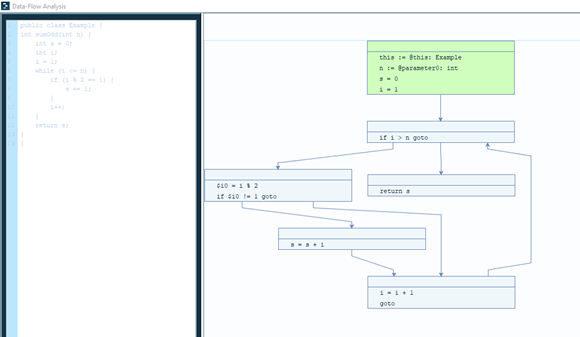
\includegraphics [scale=1] {my_folder/images/my/10}
	\caption{Результат работы VisualDFA}
	\label{fig:10}
\end{figure}

\subsection{VisualControlFlowGraph4J} \label{ch2:subsec-title-abbr}
VisualControlFlowGraph4J – инструмент для построения и визуализации Java-кода в виде CFG, использующий ANTLR и GraphViz.
Инструмент помогает строить CFG, но у него также есть ряд недостатков. Построение CFG нельзя назвать интерактивным. Он требует файла с исходным кодом в папке с ресурсами для того, чтобы строить модель по нему. Граф сохраняется в файловую систему в виде SVG-файла по завершению работы программы. В самом CFG присутствуют обозначения типов данных, что делает граф привязанным к языку программирования. Также наблюдается проблема с тем, что, смотря на стрелки, исходящие из блоков условий, непонятно, по какой из них переходить при истинном или ложном условии. Кроме того, никак не обозначены параметры метода, граф для которого строится.
VisualControlFlowGraph4J можно считать готовым решением для построения и визуализации CFG, но не лишённым своих недостатков. На рис. 2.2 изображен результат работы VisualControlFlowGraph4J.

\begin{figure}[h]
	\center
	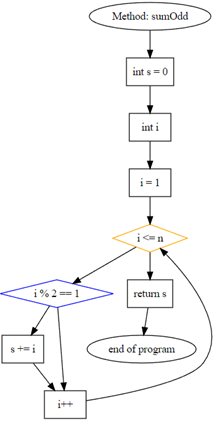
\includegraphics [scale=1.1] {my_folder/images/my/11}
	\caption{Результат работы VisualControlFlowGraph4J}
	\label{fig:11}
\end{figure}

\subsection{ANTLR} \label{ch2:subsec-title-abbr}
ANTLR (Another Tool for Language Recognition) – это мощный генератор парсеров. С его помощью можно сгенерировать парсер для любой заданной грамматики, в том числе для языков программирования. Для генерации парсера нужен файл грамматики, составленный по определённым правилам. Существует множество готовых грамматик для разных языков, в том числе для языка программирования Java. Кроме того, есть возможность вывести дерево парсинга в графическом интерфейсе.
Сам по себе ANTLR не является готовым решением для построения и визуализации AST. Он лишь может сгенерировать код по шаблону (Visitor или Listener) на одном из поддерживаемых языков программирования, который можно дописать для получения желаемого результата. Дерево парсинга, которое получается при использовании ANTLR, содержит в себе все символы исходного текста. Чтобы из этого построить AST, необходимо убрать множество лишних элементов. На рис. 2.3 изображен графический интерфейс ANTLR.

\begin{figure}[h]
	\center
	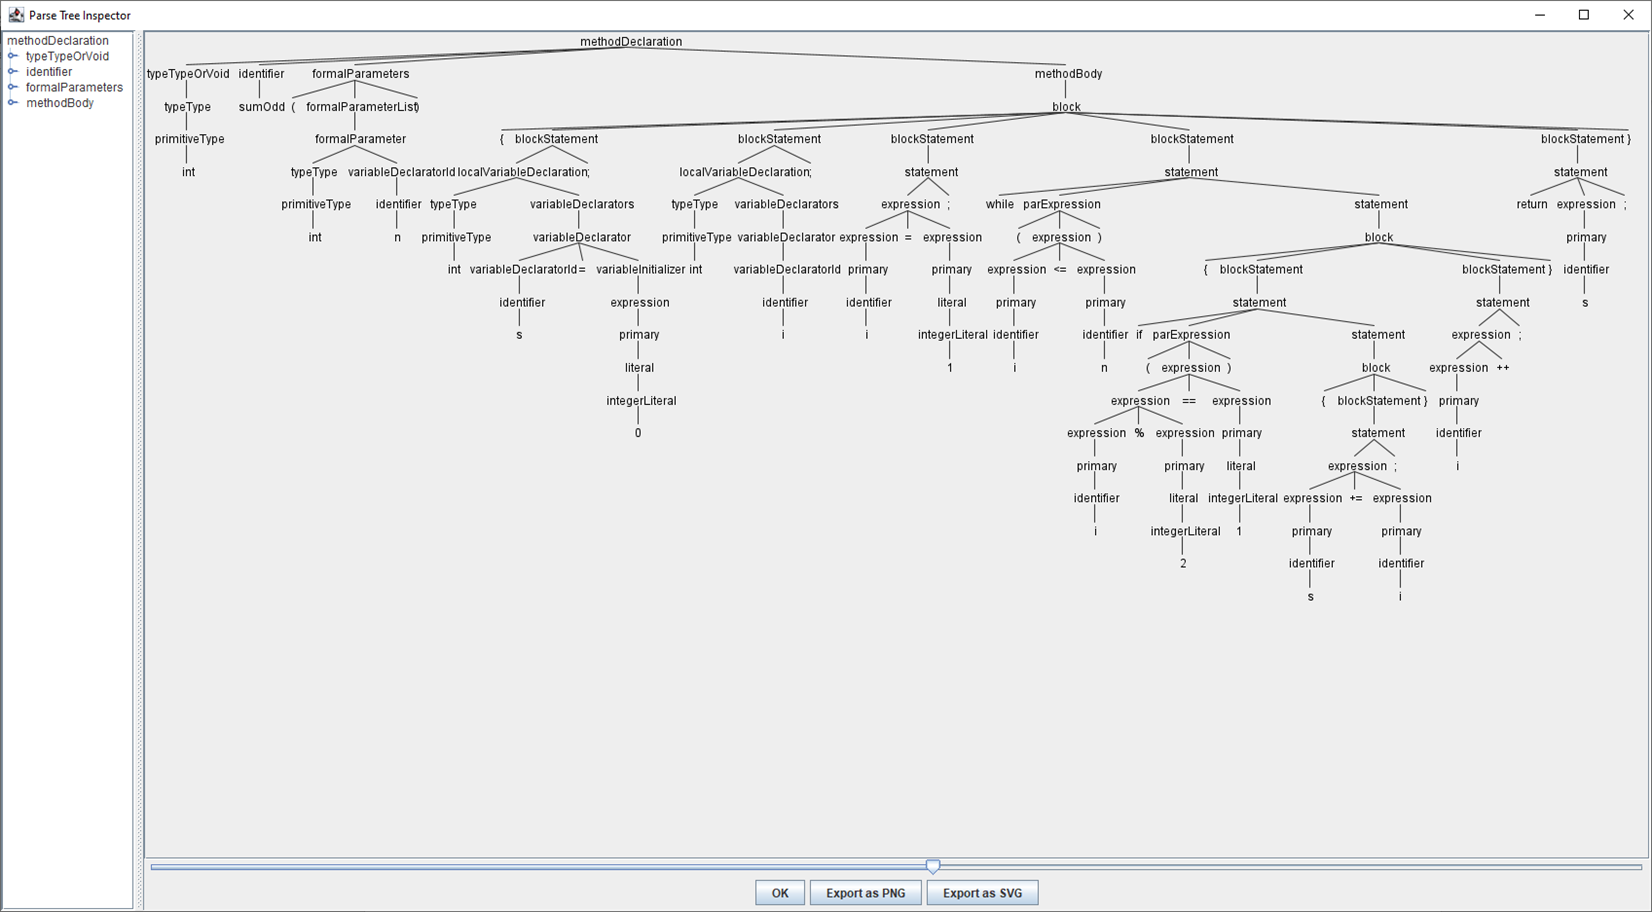
\includegraphics [scale=0.38] {my_folder/images/my/8}
	\caption{Графический интерфейс ANTLR}
	\label{fig:8}
\end{figure}

\subsection{AST Explorer} \label{ch2:subsec-title-abbr}
AST Explorer – это инструмент для парсинга кода на разных языках, в том числе Java, который использует Node.js в качестве сервера и содержит ссылки на каждый пакет в репозитории npm, используемый в качестве парсера для того или иного языка.
Из способов визуализации поддерживается только вывод в виде интерактивного иерархического текста, либо в виде кода JSON. И строится в результате не AST, а дерево парсинга, которое тоже содержит множество ненужных для построения AST узлов.
Таким образом, его тоже нельзя назвать готовым решением для построения и визуализации AST для кода на языке Java. На рис. 2.4 изображен результат работы AST Explorer.
\newpage

\begin{figure}[h]
	\center
	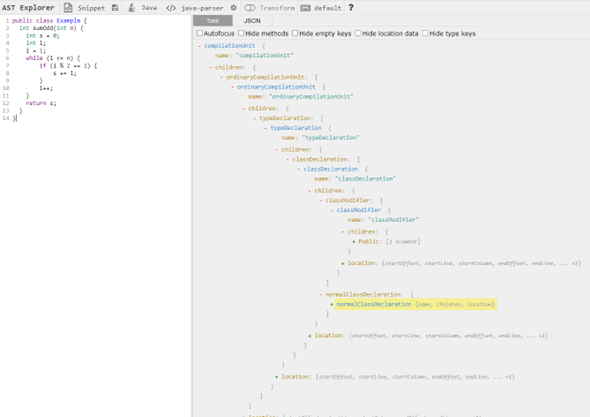
\includegraphics [scale=1] {my_folder/images/my/9}
	\caption{Результат работы AST Explorer}
	\label{fig:9}
\end{figure}

\section{Выводы по главе} \label{ch2:sec2}
В данной главе проведен обзор и анализ существующих средств визуализации моделей программ. Были найдены лишь решения для AST и CFG, для визуализации остальных моделей программ не было найдено ни одного достойного решения. Также хочется отметить, что не существует ни одного сервиса, способного интерактивно визуализировать несколько разных моделей программ. На основе результата обзора можно сделать вывод о том, что тема выпускной квалификационной работы является актуальной.
\newpage